% The archive-index system. Every statement is checked against src/archive_index (evidence level L1: code and tests).
\section{The archive-index system}\label{sec:system}

\subsection{Architecture and data flow}
archive-index keeps one SQLite database per archive. A \code{documents} table records each source file (collection, path, size, modification time, SHA-256, title, project); a \code{chunks} table holds the text fragments with their locator (page, slide, time window, frame), the embedding vector as a binary blob, and a hash of the text that produced the vector. An FTS5 virtual table indexes three columns of each chunk: the word terms described below, the body and the heading, with the \code{unicode61} tokenizer and diacritics kept. The database runs in write-ahead-log mode, so the terminal interface, the scheduled indexing jobs and ad hoc searches can read while the indexer writes.

Sources are grouped into collections: Markdown notes (\code{wiki}); office documents and PDF (\code{docs}, with \code{.doc}, \code{.rtf}, \code{.odt}, \code{.ppt} and \code{.odp} converted through LibreOffice); spreadsheets and CSV (\code{tables}); Git history; Claude and Codex agent sessions; run logs; pictures; sound; and video. Source code, configuration and log files are opt-in collections searched only when named. Markdown is split at headings and packed paragraph by paragraph into chunks of at most 1\,200 characters; a longer paragraph is split hard at that length.

\begin{figure}[p]
\centering
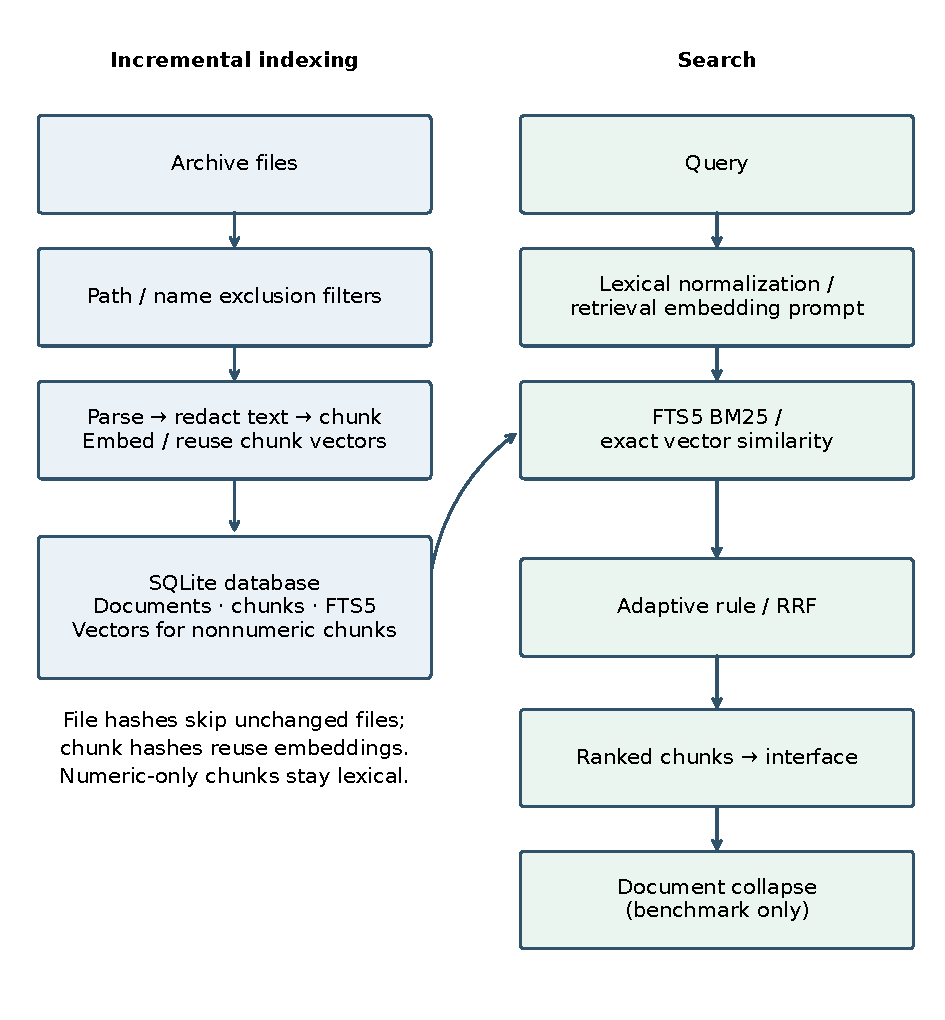
\includegraphics[width=\linewidth]{architecture.pdf}
\caption{Indexing and search data flow with the default local backend. Text redaction applies known patterns; images and audio are not content-redacted. Numeric-only chunks remain available to lexical search without vectors. Document collapse belongs to the benchmark, outside the query timer.}
\label{fig:architecture}
\end{figure}

\subsection{Lexical layer}
Words are runs of Unicode letters and digits that may be joined by a hyphen or an apostrophe, at least two characters long, lower-cased. The four apostrophe characters used in Ukrainian text (U+2019, U+02BC, U+2018 and the backtick) are mapped to the ASCII apostrophe before tokenization, so that \emph{м’ята} and \emph{мʼята} are one word. The FTS \code{terms} column stores every word followed by its normal forms from the pymorphy3 Ukrainian and Russian analyzers. A word containing a letter that exists only in Ukrainian (і, ї, є, ґ) goes through the Ukrainian analyzer only; other words go through both. When a dictionary knows the word, only dictionary normal forms are kept; the analyzers' guesses are used only for words that neither dictionary knows (Appendix~\ref{sec:intro-history} records the defect that this rule corrects).

Identifiers such as \code{36.101}, \code{19.6.0} or \code{RVZ0014A-2} (letter and digit runs joined by dots or slashes, or a hyphen followed by a digit) are matched as exact phrases, so a query for \code{36.109} never matches a document that contains only \code{36}. A query becomes an FTS5 expression in which each word is a disjunction of its surface and normal forms, the words are joined by OR, and an identifier clause, if present, is joined to the words by AND. Lexical ranking is FTS5 BM25.

\subsection{Dense layer}
The dense layer uses EmbeddingGemma~2 through SentenceTransformers, in bfloat16 on a GPU (the model card warns that float16 degrades the embeddings) and in float32 on a CPU. Documents are embedded as \code{title: <title> | text: <chunk>}; queries carry the model's retrieval prompt \code{task: search result | query:}, or \code{task: code retrieval | query:} when the code collection is searched. Vectors are L2-normalized; the 256-dimensional variant truncates them (Matryoshka truncation) and normalizes again. Pictures, PDF pages without a text layer and video frames (one every 5~s, at most 120 per video) are embedded as images in the same space. Sound is resampled to 16~kHz and embedded in 20~s windows with a 15~s step; when a transcript file accompanies a recording, the transcript lines that overlap a window become that window's text. A llama.cpp server running a GGUF build of the model is an optional text-only backend. Semantic search is exact: all vectors are held in memory and scored with one NumPy matrix--vector product, with no approximate nearest-neighbour index.

\subsection{Fusion}
Three ranking modes are available: lexical only, semantic only and hybrid. The default hybrid strategy (\sys{adaptive}) looks at the best lexical chunk. If it contains at least 90\% of the query words as whole words, the query is treated as a search for an exact phrase: only lexical results are returned, in BM25 order, except that chunks in which the query words occur in order within a slack of three words are moved to the front. Otherwise the semantic ranking comes first and the lexical results that it does not already contain follow; with no lexical match the result is purely semantic. Reciprocal-rank fusion with $k=60$ (\sys{rrf}) is the alternative hybrid strategy. In the interface, at most three chunks per document are shown, with a count of the remaining ones; benchmark runs collapse chunks to documents (Section~\ref{sec:method}).

\subsection{Incremental indexing}
A file is skipped when its size and modification time are unchanged, and also when its SHA-256 is unchanged; only then is it parsed again. Vectors are reused for chunks whose text hash is already stored, so editing a note re-embeds only the edited chunks. Files that disappeared are removed from their collection. Fragments of notes and documents with fewer than 20 letters (page numbers, punctuation) are dropped unless every fragment of the file is that short; pictures and sound are never dropped. Each run writes a report of indexed, skipped and failed files; a failure in one file does not stop the run.

\subsection{Privacy}
The default embedding backend processes document content locally. The optional llama.cpp client defaults to a loopback server; configuring an external \code{ARCHIVE\_LLAMA\_URL} sends text to that endpoint. Local processing therefore depends on the backend configuration. Directories \code{.ssh}, \code{.gnupg}, \code{.aws}, \code{.kube}, \code{.password-store}, \code{.docker} and key rings, and files whose names match key, certificate, password-store, environment and credential patterns (for example \code{*.pem}, \code{*.kdbx}, \code{id\_rsa*}, \code{.env}, \code{*secret*}, \code{*token*}) never enter the index. Inside indexed text, PEM private-key blocks, access keys in the formats of several common services (OpenAI, AWS, GitHub, Slack, bearer tokens) and explicit credential assignments such as \code{password=...} are replaced by a redaction marker before storage. The patterns cover known formats only; they are a safety net, not a guarantee. The redaction report counts kinds and never stores values.
